\documentclass[12pt,a4paper]{report}
\usepackage[utf8]{inputenc}
\usepackage[T1]{fontenc}
\usepackage{lmodern}
\usepackage[scaled]{helvet}
\renewcommand{\familydefault}{\sfdefault}
\usepackage{graphicx}
\usepackage{geometry}
\usepackage{setspace}
\usepackage{titlesec}
\usepackage{fancyhdr}
\usepackage{array}
\usepackage{float}
\usepackage{enumitem}
\usepackage{tikz}
\usetikzlibrary{arrows.meta,positioning,shapes.geometric,fit,backgrounds}
\usepackage{url}
\usepackage[hidelinks]{hyperref}
\geometry{a4paper, margin=1in, headheight=15pt}
\graphicspath{{images/}}
\emergencystretch=3em
\newcolumntype{L}[1]{>{\raggedright\arraybackslash}p{#1}}
\setlength{\parindent}{1.5em}

% Running header and footer, in the style of the department's seminar reports
\pagestyle{fancy}
\fancyhf{}
\fancyhead[L]{\small LangGraph Seminar}
\fancyhead[R]{\small\nouppercase{\leftmark}}
\fancyfoot[L]{\small B.Tech AI\&DS 2023--2027}
\fancyfoot[C]{\thepage}
\renewcommand{\headrulewidth}{0.4pt}
\fancypagestyle{plain}{%
  \fancyhf{}%
  \fancyfoot[L]{\small B.Tech AI\&DS 2023--2027}%
  \fancyfoot[C]{\thepage}%
  \renewcommand{\headrulewidth}{0pt}}

\tikzset{
  box/.style={draw, rounded corners=3pt, align=center, minimum height=1cm, inner sep=6pt, font=\small},
  layer/.style={draw, dashed, rounded corners=6pt, inner sep=10pt},
  arrow/.style={-{Stealth[length=2.5mm]}, thick},
  decision/.style={draw, diamond, aspect=2, align=center, inner sep=1pt, font=\small}
}

\begin{document}

% ------------------------------------------------------------------ Title page
\begin{titlepage}
    \begin{center}
        \vspace*{0.5cm}
        {\LARGE LangGraph: Graph-Based Orchestration for Stateful LLM Applications}\\[0.4cm]
        {\large and its Applications}\\[0.5cm]
        {\large CAQ413 Seminar}\\[1.8cm]

        {\itshape Seminar Report submitted in partial fulfillment for the degree}\\
        {\itshape B.Tech in Computer Science and Engineering (Artificial Intelligence)}\\[1.8cm]

        Submitted by\\[0.4cm]
        Nikhil Jimmy Thomas (Reg No: MUT23CA055)\\[1.2cm]

        
\includegraphics[width=0.45\textwidth]{MITS_LOGO.pdf}\\[1.2cm]

        DEPARTMENT OF ARTIFICIAL INTELLIGENCE AND DATA SCIENCE\\
        {\itshape (Affiliated to APJ Abdul Kalam Technological University)}\\[0.6cm]
        October 2026
    \end{center}
\end{titlepage}

\pagenumbering{roman}
\setcounter{page}{1}

% ------------------------------------------------------------------ Certificate
\thispagestyle{plain}
\begin{center}
    
\includegraphics[width=0.45\textwidth]{MITS_LOGO.pdf}\\[0.3cm]
    Varikoli P.O., Puthencruz-682308\\[1cm]
    DEPARTMENT OF ARTIFICIAL INTELLIGENCE \& DATA SCIENCE\\[1.5cm]
    {\Large CERTIFICATE}
\end{center}
\vspace{1cm}

\noindent This is to certify that the seminar report entitled ``LangGraph: Graph-Based Orchestration for Stateful LLM Applications and its Applications'' submitted by Nikhil Jimmy Thomas (Reg No: MUT23CA055) of Semester VII B.Tech Computer Science and Engineering (AI) is a bonafide record of the work done under my supervision during the academic year 2026--2027.

\vspace{3cm}
\noindent
\begin{tabular}{@{}L{0.28\textwidth} L{0.36\textwidth} L{0.28\textwidth}@{}}
\textbf{Guide} & \textbf{Coordinators} & \textbf{Head of the Department} \\[6pt]
Ms. Nimmi M K & Ms. Thasni K N \& Ms. Vishnupriya Vijay & Dr. Cerene Mariam Abraham \\[2pt]
Asst. Professor & Asst. Professors & Associate Professor \\[2pt]
Dept. of AI \& DS & Dept. of AI \& DS & Dept. of AI \& DS \\
\end{tabular}

% ------------------------------------------------------------------ Acknowledgements
\newpage
\thispagestyle{plain}
\begin{center}
    {\Large ACKNOWLEDGEMENTS}
\end{center}
\vspace{0.6cm}
\begin{onehalfspace}
This seminar report is the outcome of my own effort, but it would not have taken shape without the support and guidance of several people and institutions. It is now my privilege to acknowledge their contributions.

First and foremost, I would like to express my heartfelt gratitude to my seminar guide, Asst.\ Prof.\ \textit{Ms.\ Nimmi M K}, for the continuous encouragement, guidance and patience shown throughout this seminar. The suggestions I received at each stage helped me move from a broad interest in AI agents to a focused study of LangGraph. I extend my sincere thanks to my seminar coordinators, Asst.\ Prof.\ \textit{Ms.\ Thasni K N} and Asst.\ Prof.\ \textit{Ms.\ Vishnupriya Vijay}, for reviewing my work critically and offering feedback that improved both the presentation and this report.

I am also grateful to Dr.\ Cerene Mariam Abraham, Head of the Department of Artificial Intelligence and Data Science, for her constant support and for fostering an environment that encourages learning. I would like to express my sincere gratitude to Dr.\ Neelakantan P.\ C., Principal, for his guidance and for the academic framework that made this seminar possible.

I am thankful to the management of Muthoot Institute of Technology \& Science for the facilities and resources provided, and to all the faculty and staff of the Artificial Intelligence and Data Science Department for a supportive learning environment.

I also remain indebted to my friends and classmates of S7 CSAI, whose discussions, questions and company made this work more enjoyable. Finally, I thank everyone who, knowingly or unknowingly, contributed to the completion of this seminar report.
\end{onehalfspace}

\vspace{1.5cm}
\begin{flushright}
Nikhil Jimmy Thomas\\
(Reg.\ No: MUT23CA055)
\end{flushright}

% ------------------------------------------------------------------ Abstract
\newpage
\thispagestyle{plain}
\begin{center}
    {\Large Abstract}
\end{center}
\vspace{0.6cm}
\begin{onehalfspace}
Large language models (LLMs) can now reason, write text and call external tools, but most real tasks need more than a single model call. They need several steps, decisions about what to do next, retries when something goes wrong, and memory of what has already happened. Simple prompt chains run in a fixed order and cannot loop, while free-running agents are flexible but hard to control and debug. LangGraph, an open-source library from LangChain Inc., takes a middle path: the developer draws the application as a graph of nodes (steps) and edges (transitions) that share one state object, and the LLM does its work inside each node. This seminar studies LangGraph through the base paper by Duan and Wang, ``Exploration of LLM Multi-Agent Application Implementation Based on LangGraph+CrewAI'' (arXiv:2411.18241, 2024). The paper combines LangGraph, which controls the flow of a multi-agent application, with CrewAI, which organises role-based agents into a team. It illustrates the combination with three cases: an email assistant that checks, drafts and sends replies, a code generation and code review loop, and an automatic work-order (ticket) auditing system. The report explains LangGraph's core concepts, reviews six related papers on LLM agents, describes the architecture and workflow proposed in the base paper, and discusses its findings, advantages, limitations and applications. A key observation is that the paper's results are qualitative case studies rather than measured benchmarks, which leaves room for future evaluation.
\end{onehalfspace}

\vspace{0.5cm}
\noindent\textbf{Keywords:} LangGraph, CrewAI, Large Language Models, Multi-Agent Systems, Agent Orchestration, Generative AI.

% ------------------------------------------------------------------ Lists
\newpage
\tableofcontents
\newpage
\listoffigures
\addcontentsline{toc}{chapter}{List of Figures}
\newpage
\listoftables
\addcontentsline{toc}{chapter}{List of Tables}

\newpage
\chapter*{List of Abbreviations}
\addcontentsline{toc}{chapter}{List of Abbreviations}
\markboth{List of Abbreviations}{}
\begin{tabular}{@{}L{3cm}L{11cm}@{}}
AI & Artificial Intelligence \\
API & Application Programming Interface \\
CoT & Chain of Thought \\
FAISS & Facebook AI Similarity Search \\
HITL & Human-in-the-Loop \\
JS / TS & JavaScript / TypeScript \\
LLM & Large Language Model \\
MAS & Multi-Agent System \\
MIT & Massachusetts Institute of Technology (licence) \\
ML & Machine Learning \\
PM & Product Manager \\
RAG & Retrieval-Augmented Generation \\
SDG & Sustainable Development Goal \\
SOP & Standard Operating Procedure \\
\end{tabular}

\newpage
\pagenumbering{arabic}
\setcounter{page}{1}
\onehalfspacing

% ================================================================== Chapter 1
\chapter{Introduction}

Large language models have moved quickly from answering single questions to acting as the ``brain'' of software systems. A modern LLM can reason through a problem, write code, search the web and call other tools. Yet anyone who has tried to build something useful with one runs into the same problem: real tasks need many steps. A customer query may have to be classified, routed to the right department, answered with information from a database, and then checked before it is sent. A piece of generated code has to be run, tested and fixed, possibly several times.

These workflows are not straight lines. They \textbf{branch} (if the query is about billing, go one way; otherwise, another), they \textbf{loop} (retry until the answer is correct) and they need to \textbf{remember} earlier results. Two common ways of building LLM applications both struggle here. \emph{Simple chains} run a fixed, one-way sequence of steps: they are predictable but cannot loop and have no shared state. \emph{Free-running agents} let the LLM decide everything, including which tool to call next and when to stop: they are flexible but hard to control, test and debug, and a single wrong decision can derail the whole run.

LangGraph sits between these two extremes. It is an open-source library released by LangChain Inc.\ in 2024 under the MIT licence, available for Python and JavaScript/TypeScript \cite{langgraphdocs}. Its design is inspired by graph-processing models such as Google's Pregel \cite{malewicz2010pregel} and Apache Beam. In LangGraph, the developer draws the application as a \textbf{graph}: each node is a step of work, each edge is a transition, and every node reads and updates one shared \textbf{state}. The developer decides which paths are allowed; the LLM does the work inside each step. The library works with any model provider, including OpenAI, Anthropic, Google and open-source models, and is used for single agents, multi-agent teams, retrieval-augmented generation (RAG) pipelines and workflows that need human approval.

The base paper for this seminar, by Duan and Wang \cite{duan2024langgraphcrewai}, explores what happens when LangGraph is combined with CrewAI \cite{crewaidocs}, a framework for organising role-based agents into a team. In their design, LangGraph owns the control flow (the order of steps, branching, loops and state), and CrewAI owns the teamwork (which agent does which task and how agents collaborate). The authors demonstrate this combination on an email assistant, a code generation and review loop, and a ticket-processing system.

\section*{Objectives of the Seminar}
\begin{itemize}
    \item To understand why multi-step LLM applications need explicit orchestration, and where chains and free-running agents fall short.
    \item To explain LangGraph's core concepts: state, nodes, edges, conditional edges and checkpoints.
    \item To review related work on LLM agents and multi-agent systems.
    \item To study the LangGraph+CrewAI architecture, workflow and case studies presented in the base paper.
    \item To assess the advantages, limitations and applications of graph-based agent orchestration.
\end{itemize}

The rest of this report is organised as follows. Chapter~2 reviews related literature. Chapter~3 describes the tools and frameworks involved. Chapter~4 presents the methodology of the base paper, and Chapter~5 discusses its results. Chapters~6 to 8 cover advantages, disadvantages and applications, and Chapter~9 concludes the report.

% ================================================================== Chapter 2
\chapter{Literature Survey}

This chapter summarises six studies that shaped the area of LLM agents and that help explain why a framework like LangGraph is needed. For each paper I note the method, what it showed, and the limitation that matters for building controllable multi-agent systems.

\section{ReAct: Synergizing Reasoning and Acting in Language Models (Yao et al., 2023)}

Yao et al.\ \cite{yao2023react} proposed ReAct, in which the LLM alternates between three kinds of output: a \emph{Thought} (reasoning about what to do), an \emph{Action} (calling a tool such as a Wikipedia search) and an \emph{Observation} (the tool's result). Interleaving reasoning with actions let the model gather facts as it went, and ReAct outperformed reasoning-only and acting-only baselines on HotpotQA, ALFWorld and WebShop. ReAct is now the basic pattern behind most tool-using agents. Its weakness is structural: it is a single linear loop with no persistent state, so a wrong step early in the run can cascade and derail the entire task.

\section{Reflexion: Language Agents with Verbal Reinforcement Learning (Shinn et al., 2023)}

Reflexion \cite{shinn2023reflexion} lets an agent learn from its mistakes without any fine-tuning. After a failed attempt, the agent writes a short verbal reflection on what went wrong and stores it in memory, and the reflection is fed into the next attempt. This simple idea produced large gains on coding and decision-making benchmarks. However, Reflexion depends on a reliable success or failure signal, which many real tasks do not provide, and every retry costs additional LLM calls and time.

\section{AutoGen: Enabling Next-Gen LLM Applications via Multi-Agent Conversation (Wu et al., 2023)}

AutoGen \cite{wu2023autogen}, an open-source framework from Microsoft, builds applications from several agents that solve a task by chatting with each other. Agents can combine LLMs, tools and human input, which makes the framework very flexible. The drawback is that the control flow emerges from the conversation itself. As a result, it is hard to predict what the system will do, and agents can loop or drift away from the task without strict control.

\section{MetaGPT: Meta Programming for a Multi-Agent Collaborative Framework (Hong et al., 2024)}

MetaGPT \cite{hong2024metagpt} encodes Standard Operating Procedures (SOPs) from human software teams into prompts. Agents take on roles such as product manager, architect and engineer and work like an assembly line, passing structured documents to each other and cross-checking outputs to reduce errors. MetaGPT showed that structure reduces the inconsistency of chat-based teams. However, its pipeline is fixed and designed mainly for software projects, and using many agents leads to a high token cost.

\section{A Survey on Large Language Model based Autonomous Agents (Wang et al., 2023)}

Wang et al.\ \cite{wang2023survey} reviewed the fast-growing literature on LLM-based autonomous agents and proposed a unified framework with four modules: \emph{profile} (the agent's role), \emph{memory}, \emph{planning} and \emph{action}. The survey also covers applications and evaluation methods. It is a valuable map of the field, but as a survey it offers no implementation or orchestration tool, and the field is moving faster than surveys can track.

\section{Agent AI with LangGraph: A Modular Framework for Enhancing Machine Translation Using LLMs (Wang and Duan, 2024)}

In earlier work by the same authors as the base paper \cite{wang2024translation}, LangGraph analyses the input text and routes it to a specialised translation agent, with separate agents for English, French and Japanese running on models such as GPT-4o. The paper shows LangGraph's routing in a concrete application. Its evaluation, however, covers only a few languages and is small in scale, and the system relies on a paid proprietary model.

\section*{Summary}

Taken together, these studies show steady progress: agents that act (ReAct), agents that learn from failure (Reflexion), agents that converse (AutoGen) and agents that follow procedures (MetaGPT). They also show a recurring gap. Either the flow is rigid and cannot loop or branch, or it is left to the model and becomes hard to control. What is missing is a way for the developer to define the allowed paths explicitly, with shared state, loops and recovery, while still letting the LLM do the intelligent work inside each step. This is the gap that LangGraph, and the LangGraph+CrewAI combination in the base paper, sets out to fill.

\begin{table}[H]
\centering
\renewcommand{\arraystretch}{1.3}
\caption{Summary of the literature survey}
\label{tab:lit}
\small
\begin{tabular}{|L{3.4cm}|L{5.2cm}|L{5.2cm}|}
\hline
\textbf{Paper} & \textbf{Key idea} & \textbf{Limitation} \\\hline
ReAct \cite{yao2023react} & Interleaves reasoning steps with tool actions & One linear loop; no saved state; errors cascade \\\hline
Reflexion \cite{shinn2023reflexion} & Agent reflects on failures and retries & Needs good feedback; extra LLM calls \\\hline
AutoGen \cite{wu2023autogen} & Agents solve tasks by conversing & Conversation-driven flow is hard to control \\\hline
MetaGPT \cite{hong2024metagpt} & Role-based agents follow SOPs & Rigid pipeline built for software tasks \\\hline
Agent Survey \cite{wang2023survey} & Unified framework: profile, memory, planning, action & No concrete orchestration tool \\\hline
LangGraph MT \cite{wang2024translation} & LangGraph routes text to translation agents & Few languages; small evaluation \\\hline
\end{tabular}
\end{table}

% ================================================================== Chapter 3
\chapter{Materials and Methods}

Unlike a model-training study, the base paper does not use a dataset. Its ``materials'' are the frameworks and tools from which the multi-agent system is built. This chapter describes them and the criteria the paper uses to judge the result.

\section{LangGraph: Core Concepts}

LangGraph is a framework for building stateful, multi-step LLM applications as graphs \cite{langgraphdocs}. Compared with other LLM frameworks, it offers three things the base paper highlights: \textbf{loops}, \textbf{controllability} and \textbf{persistent memory} \cite{duan2024langgraphcrewai}. It supports many kinds of control flow (single-agent, multi-agent, hierarchical and sequential) and is meant to handle complex, real-world scenarios. The building blocks are listed below and shown in Fig.~\ref{fig:graph}.

\begin{itemize}
    \item \textbf{State:} shared data, usually a typed dictionary, that every node reads and updates. Reducer functions define how an update is merged, for example appending to a list of messages instead of overwriting it.
    \item \textbf{Node:} an ordinary Python function that performs one step of work, such as calling the LLM or a tool, and returns the parts of the state it changes.
    \item \textbf{Edge:} a fixed transition: after node A, run node B.
    \item \textbf{Conditional edge:} a router function that looks at the current state and picks the next node. This is how branching and loops are expressed.
    \item \textbf{START and END:} special entry and exit points of the graph.
    \item \textbf{Checkpointer:} saves the state after every step, so a run can be paused, inspected, resumed after a crash, or continued after a human approves it.
\end{itemize}

\begin{figure}[H]
\centering
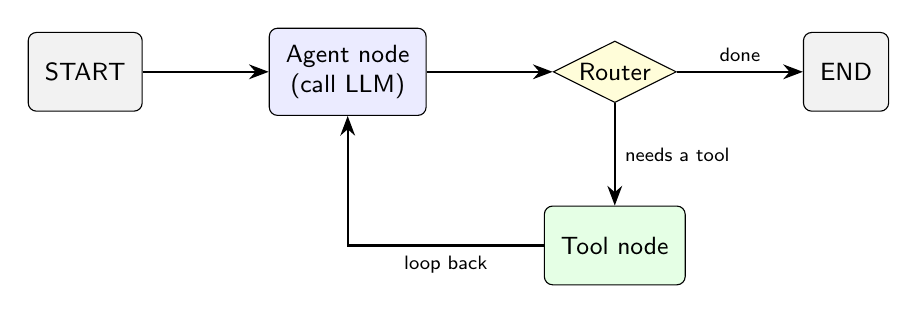
\begin{tikzpicture}[node distance=1.2cm and 1.6cm]
  \node[box, fill=gray!10] (start) {START};
  \node[box, right=of start, fill=blue!8] (agent) {Agent node\\(call LLM)};
  \node[decision, right=of agent, fill=yellow!15] (router) {Router};
  \node[box, below=1.3cm of router, fill=green!10] (tool) {Tool node};
  \node[box, right=of router, fill=gray!10] (end) {END};
  \draw[arrow] (start) -- (agent);
  \draw[arrow] (agent) -- (router);
  \draw[arrow] (router) -- node[above, font=\scriptsize]{done} (end);
  \draw[arrow] (router) -- node[right, font=\scriptsize]{needs a tool} (tool);
  \draw[arrow] (tool) -| node[below, pos=0.25, font=\scriptsize]{loop back} (agent);
\end{tikzpicture}
\caption{A minimal LangGraph agent: nodes, a conditional edge (router) and a loop}
\label{fig:graph}
\end{figure}

Building a LangGraph application takes five steps: (1) define the state, (2) add nodes as functions, (3) connect them with edges, (4) compile the graph and (5) invoke it. The following minimal example answers a question with one LLM call:

\begin{singlespace}
\small
\begin{verbatim}
from typing import TypedDict
from langgraph.graph import StateGraph, START, END

class State(TypedDict):          # 1. define the state
    question: str
    answer: str

def answer(state: State):        # 2. a node is a plain function
    return {"answer": llm.invoke(state["question"])}

g = StateGraph(State)
g.add_node("answer", answer)
g.add_edge(START, "answer")      # 3. connect edges
g.add_edge("answer", END)
app = g.compile()                # 4. compile
app.invoke({"question": "What is LangGraph?"})   # 5. run
\end{verbatim}
\end{singlespace}

\section{CrewAI Framework}

CrewAI \cite{crewaidocs} is an open-source framework for coordinating role-playing, autonomous AI agents so that they can cooperate on complex problems. Developers define each agent with a specific role, objective and set of tools. Its four building blocks are:

\begin{itemize}
    \item \textbf{Agent:} an autonomous unit that can perform tasks, make decisions and communicate with other agents. It is defined by a role, a goal and a backstory.
    \item \textbf{Task:} a specific piece of work carried out by an agent, including its description, the agent that executes it and the tools it needs.
    \item \textbf{Tool:} a capability an agent can use, such as reading email or searching documents.
    \item \textbf{Crew:} a team of agents together with the process that orchestrates their tasks.
\end{itemize}

CrewAI supports APIs such as OpenAI and Ollama, and its key features include role-customised agents, automatic task delegation and flexible task management \cite{duan2024langgraphcrewai}. It is aimed at multi-step workflows, decision-making and problem-solving.

\section{Development Environment}

The base paper builds its application cases with the following components \cite{duan2024langgraphcrewai}:

\begin{table}[H]
\centering
\renewcommand{\arraystretch}{1.3}
\caption{Development environment used in the base paper}
\label{tab:env}
\begin{tabular}{|L{3.8cm}|L{3cm}|L{7cm}|}
\hline
\textbf{Component} & \textbf{Tool} & \textbf{Purpose} \\\hline
Multi-agent framework & CrewAI & Organising and coordinating collaborative work among AI agents \\\hline
Graph workflow & LangGraph & Managing state sharing and process control between graph nodes \\\hline
Workflow tracking & LangSmith \cite{langsmith} & Monitoring and auditing the execution of workflows \\\hline
Embedding model & Ollama embeddings & Converting work-order text into vectors for retrieval \\\hline
Vector database & FAISS \cite{johnson2019faiss} & Storing and retrieving vectors, which speeds up data access \\\hline
\end{tabular}
\end{table}

\section{Evaluation Criteria}

The base paper is an exploratory case study. It does not report accuracy, latency or cost figures. Instead, it judges the LangGraph+CrewAI combination qualitatively, on four criteria that also guide this report:

\begin{itemize}
    \item \textbf{Controllability:} whether the developer can define and restrict the flow of the application precisely.
    \item \textbf{Information flow:} how efficiently state and results pass between agents and steps.
    \item \textbf{Collaboration:} how well work is divided among agents with different roles.
    \item \textbf{Extensibility:} how easily existing tools and agents, for example those built with LangChain, can be integrated.
\end{itemize}

% ================================================================== Chapter 4
\chapter{Methodology}

\section{Design Rationale}

The base paper starts from a simple observation: complex tasks are too much for a single LLM agent, and multi-agent systems need two things to work well, namely precise control of the flow and good teamwork \cite{duan2024langgraphcrewai}. Rather than making one framework do both, the authors give each job to the framework best suited to it. LangGraph's graph architecture provides precise control and efficient information flow between agents. CrewAI's role-based crews provide intelligent task allocation and resource management. The paper studies two questions: (1) how to design the architecture of agents on LangGraph for more precise control, and (2) how to enhance agents with CrewAI so that they can complete different tasks.

\section{System Architecture}

The architecture has two layers that meet at the shared state (Fig.~\ref{fig:arch}).

\begin{itemize}
    \item \textbf{LangGraph, the control layer.} The user's task enters the graph. Nodes represent agent steps, and edges with conditional routing decide which step runs next. The shared state carries data between steps.
    \item \textbf{CrewAI, the team layer.} Inside a node, a crew of agents does the actual work. Each agent has a role and a goal, tasks are assigned to agents, and the agents collaborate to produce the node's result.
\end{itemize}

\begin{figure}[H]
\centering
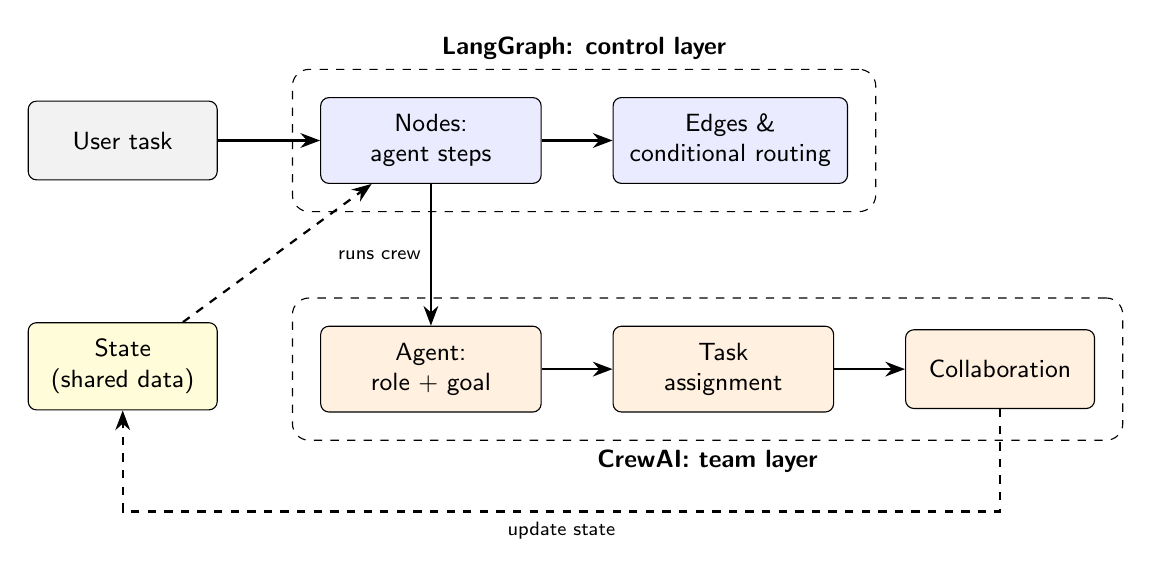
\begin{tikzpicture}[node distance=0.9cm and 0.9cm]
  \node[box, fill=gray!10, minimum width=2.4cm] (task) {User task};
  \node[box, right=1.3cm of task, fill=blue!8, minimum width=2.8cm] (nodes) {Nodes:\\agent steps};
  \node[box, right=of nodes, fill=blue!8, minimum width=2.8cm] (edges) {Edges \&\\conditional routing};
  \node[box, below=1.8cm of nodes, fill=orange!12, minimum width=2.8cm] (agent) {Agent:\\role + goal};
  \node[box, right=of agent, fill=orange!12, minimum width=2.8cm] (assign) {Task\\assignment};
  \node[box, right=of assign, fill=orange!12, minimum width=2.4cm] (collab) {Collaboration};
  \node[box, below=1.8cm of task, fill=yellow!15, minimum width=2.4cm] (state) {State\\(shared data)};
  \begin{scope}[on background layer]
    \node[layer, fit=(nodes)(edges), label={[font=\small\bfseries]above:LangGraph: control layer}] (lg) {};
    \node[layer, fit=(agent)(assign)(collab), label={[font=\small\bfseries]below:CrewAI: team layer}] (cr) {};
  \end{scope}
  \draw[arrow] (task) -- (nodes);
  \draw[arrow] (nodes) -- (edges);
  \draw[arrow] (nodes) -- node[left, font=\scriptsize]{runs crew} (agent);
  \draw[arrow] (agent) -- (assign);
  \draw[arrow] (assign) -- (collab);
  \draw[arrow, dashed] (state) -- (nodes);
  \draw[arrow, dashed] (collab.south) -- ++(0,-1.3) -| node[below, pos=0.25, font=\scriptsize]{update state} (state.south);
\end{tikzpicture}
\caption{Two-layer architecture: LangGraph controls the flow, CrewAI performs the work inside each node}
\label{fig:arch}
\end{figure}

\section{Integrating LangGraph with CrewAI}

According to the authors, the integrated framework is a powerful tool for complex task management. It optimises task execution through flexible workflows, collaboration between agents and graph-structured management. It also supports custom development by integrating with existing tools. CrewAI keeps the process efficient through clear task allocation and role definitions, and because it integrates with LangChain, developers who already use LangChain can bring in their existing agents with little effort \cite{duan2024langgraphcrewai}.

In practice, the division of labour is straightforward:
\begin{itemize}
    \item \textbf{LangGraph owns the control flow:} the order of steps, branching, loops and state.
    \item \textbf{CrewAI owns the teamwork:} which role-based agent does which task, and how the agents collaborate.
\end{itemize}

\section{Workflow}

Fig.~\ref{fig:workflow} shows how a task moves through the combined system. LangGraph receives the task and routes it to the next node. The CrewAI crew in that node performs the task, and the result is written back to the shared state. A conditional edge then checks whether the work is complete. If it is not, the flow loops to the next step; if it is, the graph ends.

\begin{figure}[H]
\centering
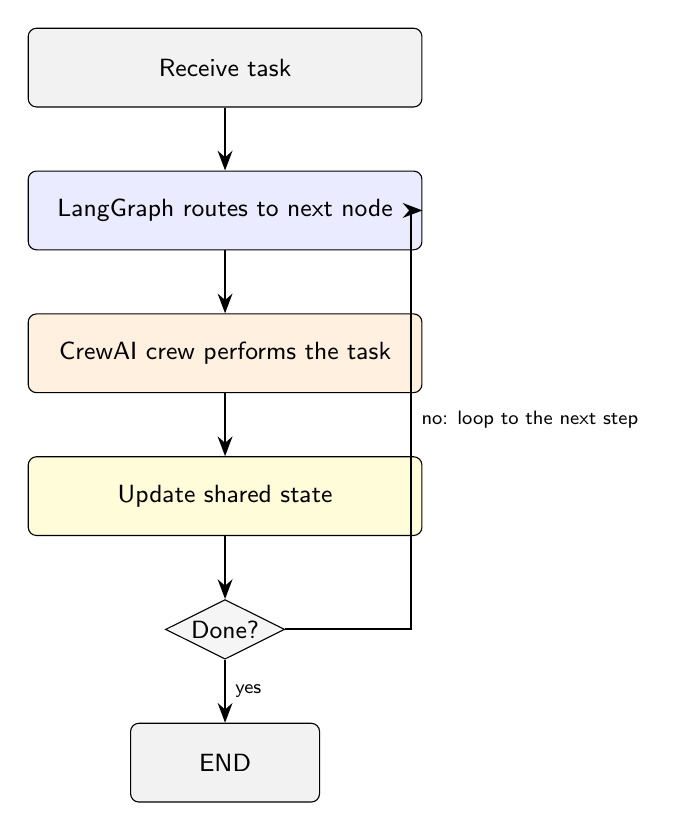
\begin{tikzpicture}[node distance=0.8cm]
  \node[box, fill=gray!10, minimum width=5cm] (recv) {Receive task};
  \node[box, below=of recv, fill=blue!8, minimum width=5cm] (route) {LangGraph routes to next node};
  \node[box, below=of route, fill=orange!12, minimum width=5cm] (crew) {CrewAI crew performs the task};
  \node[box, below=of crew, fill=yellow!15, minimum width=5cm] (upd) {Update shared state};
  \node[decision, below=of upd, fill=gray!8] (done) {Done?};
  \node[box, below=of done, fill=gray!10, minimum width=2.4cm] (end) {END};
  \draw[arrow] (recv) -- (route);
  \draw[arrow] (route) -- (crew);
  \draw[arrow] (crew) -- (upd);
  \draw[arrow] (upd) -- (done);
  \draw[arrow] (done) -- node[right, font=\scriptsize]{yes} (end);
  \draw[arrow] (done.east) -- ++(1.6,0) |- node[right, pos=0.25, font=\scriptsize]{no: loop to the next step} (route.east);
\end{tikzpicture}
\caption{Workflow of the LangGraph+CrewAI system}
\label{fig:workflow}
\end{figure}

\section{Worked Example: Automatic Email Handling}

To make the method concrete, the base paper takes the automatic email composition and sending example from the CrewAI website and rebuilds it on LangGraph+CrewAI \cite{duan2024langgraphcrewai}. The task is broken into manageable steps, and their execution is automated.

Fig.~\ref{fig:email} shows the graph. The flow starts at \texttt{check\_new\_emails}. A conditional edge either continues to \texttt{draft\_responses}, when there are new emails, or goes straight to \texttt{wait\_next\_run}. After waiting, the graph loops back to check again. The loop, which a simple chain cannot express, is what turns a one-off script into a continuously running assistant.

\begin{figure}[H]
\centering
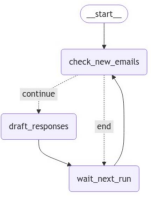
\includegraphics[width=0.38\textwidth]{bp_fig1_email_graph.png}
\caption{Email workflow graph built with LangGraph+CrewAI (source: Duan and Wang \cite{duan2024langgraphcrewai}, Fig.~1)}
\label{fig:email}
\end{figure}

The code that builds this graph (Fig.~\ref{fig:code}) follows the five steps described in Chapter~3. The interesting line is the node \texttt{draft\_responses}, whose function is \texttt{EmailFilterCrew().kickoff}. Here an entire CrewAI crew runs as a single LangGraph node:

\begin{singlespace}
\small
\begin{verbatim}
workflow = StateGraph(EmailsState)
workflow.add_node("check_new_emails", nodes.check_email)
workflow.add_node("wait_next_run", nodes.wait_next_run)
workflow.add_node("draft_responses", EmailFilterCrew().kickoff)
workflow.set_entry_point("check_new_emails")
workflow.add_conditional_edges(
    "check_new_emails", nodes.new_emails,
    {"continue": "draft_responses", "end": "wait_next_run"})
workflow.add_edge("draft_responses", "wait_next_run")
workflow.add_edge("wait_next_run", "check_new_emails")
self.app = workflow.compile()
\end{verbatim}
\end{singlespace}

\begin{figure}[H]
\centering
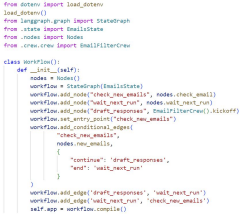
\includegraphics[width=0.7\textwidth]{bp_fig2_code.png}
\caption{LangGraph+CrewAI workflow code (source: \cite{duan2024langgraphcrewai}, Fig.~2)}
\label{fig:code}
\end{figure}

Inside the crew, each agent is defined by its role, goal and backstory (Fig.~\ref{fig:agent}). For example, the ``Senior Email Analyst'' filters out newsletters and promotional mail. A task (Fig.~\ref{fig:task}) then describes exactly what the agent must do, which output format is expected, and which agent performs it.

\begin{figure}[H]
\centering
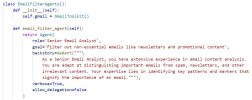
\includegraphics[width=0.75\textwidth]{bp_fig3_agent.png}
\caption{Agent definition in CrewAI (source: \cite{duan2024langgraphcrewai}, Fig.~3)}
\label{fig:agent}
\end{figure}

\begin{figure}[H]
\centering
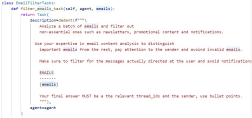
\includegraphics[width=0.75\textwidth]{bp_fig4_task.png}
\caption{Task definition in CrewAI (source: \cite{duan2024langgraphcrewai}, Fig.~4)}
\label{fig:task}
\end{figure}

% ================================================================== Chapter 5
\chapter{Results and Performance}

The base paper reports its results as application case studies. It shows that the LangGraph+CrewAI design can be used to build working multi-agent applications and describes what the combination improves. This chapter presents those cases, the key findings and a discussion of what the results do and do not show.

\section{Application Case 1: Code Generation with Code Review}

Using LangGraph+CrewAI, the authors built a multi-agent application that combines code generation with code review (Fig.~\ref{fig:codegen}). A question goes to a \emph{code generation} node, which produces code. A \emph{code check} node then tests it. If the check fails, the flow loops back to generation with the feedback; if it passes, the code is returned as the solution. Because status data and feedback are shared in real time through the graph state, the authors report that the efficiency of code generation improved \cite{duan2024langgraphcrewai}. This is the same write, test and fix loop that the Reflexion and ReAct papers motivate, but here the loop is an explicit, inspectable edge in the graph rather than something left to the model.

\begin{figure}[H]
\centering
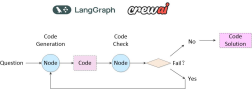
\includegraphics[width=0.7\textwidth]{bp_fig5_codegen.png}
\caption{Code generation and code check loop based on LangGraph+CrewAI (source: \cite{duan2024langgraphcrewai}, Fig.~5)}
\label{fig:codegen}
\end{figure}

\section{Application Case 2: Automatic Work-Order Processing}

The second case automates the auditing and forwarding of work orders, or tickets (Fig.~\ref{fig:tickets}). The text of each ticket is converted into vectors with an Ollama embedding model and stored in FAISS, so that similar past tickets can be retrieved. Several CrewAI agents, each with its own task, then analyse the ticket in depth. By sharing their understanding of the content, the agents can interpret tickets more accurately, and the authors report that this improved the efficiency of ticket processing \cite{duan2024langgraphcrewai}.

\begin{figure}[H]
\centering
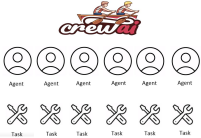
\includegraphics[width=0.5\textwidth]{bp_fig6_tickets.png}
\caption{Work-order processing with a crew of agents and tasks (source: \cite{duan2024langgraphcrewai}, Fig.~6)}
\label{fig:tickets}
\end{figure}

\section{Key Findings}

From these cases, the authors draw four findings:
\begin{itemize}
    \item \textbf{Efficient information flow:} LangGraph's graph architecture improves how efficiently information passes between agents.
    \item \textbf{Precise control:} designing agents on LangGraph gives precise control over the multi-agent workflow.
    \item \textbf{Better collaboration:} CrewAI's intelligent task allocation and resource management improve teamwork and system performance.
    \item \textbf{Complex tasks:} agents divide the work and collaborate on tasks that a single agent struggles with.
\end{itemize}

\section{Comparison with Other Approaches}

Table~\ref{tab:compare} compares the approaches discussed in this report on the properties that matter for building controllable multi-agent applications. The comparison is qualitative and based on the literature reviewed in Chapter~2.

\begin{table}[H]
\centering
\renewcommand{\arraystretch}{1.3}
\caption{Qualitative comparison of LLM application approaches}
\label{tab:compare}
\footnotesize
\begin{tabular}{|L{2.4cm}|L{1.7cm}|L{1.2cm}|L{1.8cm}|L{1.7cm}|L{1.7cm}|L{1.9cm}|}
\hline
\textbf{Approach} & \textbf{Flow defined by} & \textbf{Loops} & \textbf{Persistent state} & \textbf{Human-in-the-loop} & \textbf{Role-based teamwork} & \textbf{Predictability} \\\hline
Simple chain & Developer & No & No & No & No & High \\\hline
ReAct agent & LLM & Yes & No & Limited & No & Low \\\hline
AutoGen & Conversation & Yes & Partial & Yes & Yes & Low \\\hline
MetaGPT & Fixed SOP & Limited & Documents & No & Yes & Medium \\\hline
LangGraph alone & Developer (graph) & Yes & Yes (checkpoints) & Yes & Manual & High \\\hline
\textbf{LangGraph + CrewAI} & \textbf{Developer (graph)} & \textbf{Yes} & \textbf{Yes} & \textbf{Yes} & \textbf{Yes (crews)} & \textbf{High} \\\hline
\end{tabular}
\end{table}

\section{Discussion}

The base paper succeeds in showing \emph{how} LangGraph and CrewAI fit together, and its three cases make the division of responsibilities easy to understand: the graph decides what happens next, and the crew decides who does it. The examples are also practical. Email triage, code review and ticket handling are everyday tasks in many organisations.

At the same time, the results should be read for what they are. The paper reports no quantitative measurements: no accuracy or success rates, no latency or cost figures, and no comparison against a single-agent baseline or another framework. Claims such as ``improved efficiency'' are therefore based on the authors' observation of the cases, not on measured experiments. A natural next step would be to evaluate the combined framework on a benchmark, for example measuring the task success rate, the number of LLM calls and the cost against a single agent and against LangGraph alone. Even so, the paper is a useful and approachable guide to designing multi-agent applications in which control and collaboration are handled by separate, well-defined layers.

% ================================================================== Chapter 6
\chapter{Advantages}

\begin{itemize}
    \item \textbf{Explicit control:} the developer decides which paths the application may take. The LLM fills in each step but cannot invent a new flow, which makes behaviour easier to predict and to audit.
    \item \textbf{Shared state:} every step sees the same up-to-date data, so information does not have to be copied between agents or squeezed into prompts.
    \item \textbf{Loops and retries:} a step can be repeated until a condition is met, for example regenerating code until its tests pass. Plain chains cannot do this.
    \item \textbf{Persistence:} checkpointers save the state after every step, so an application can pause, resume and recover after a failure without starting over.
    \item \textbf{Human-in-the-loop:} the graph can stop at any node and wait for a person to review or edit the state before continuing, which is important for sensitive actions such as sending emails.
    \item \textbf{Easy to debug:} each node is a plain function that can be tested and traced on its own. Tools such as LangSmith show exactly which path a run took.
    \item \textbf{Model-agnostic:} LangGraph and CrewAI both work with many LLM providers, including OpenAI, Anthropic, Google and local models through Ollama.
    \item \textbf{Clear teamwork with CrewAI:} roles, goals and tasks give each agent a well-defined job, and existing LangChain agents can be brought into a crew with little effort.
\end{itemize}

% ================================================================== Chapter 7
\chapter{Disadvantages}

\begin{itemize}
    \item \textbf{Learning curve:} graphs, typed state, reducers and checkpointers take time to learn, and combining two frameworks adds a second set of concepts.
    \item \textbf{More code for simple tasks:} a task that a basic chain handles in a few lines needs more setup as a graph.
    \item \textbf{Large graphs get complex:} with many nodes and conditional routes, the flow becomes hard to visualise and reason about.
    \item \textbf{Cost and latency:} loops and multiple agents mean more LLM calls, which increases both the running cost and the response time.
    \item \textbf{Still depends on the LLM:} the graph constrains the paths, but a wrong model output can still pick a wrong route or produce a poor result inside a node.
    \item \textbf{Fast-changing ecosystem:} the APIs of both frameworks change between versions, so code and tutorials go out of date quickly.
    \item \textbf{No quantitative evaluation in the base paper:} the benefits are shown through case studies, so they are not yet backed by measured results.
\end{itemize}

% ================================================================== Chapter 8
\chapter{Applications}

\begin{itemize}
    \item \textbf{Customer support:} a router node classifies each query and sends it to a billing agent, a technical agent or a human, with the conversation kept in the shared state.
    \item \textbf{RAG question answering:} the graph retrieves documents, grades their relevance and, if they are poor, rewrites the query and searches again before answering.
    \item \textbf{Code generation and bug fixing:} write, test and fix in a loop, as in the base paper's code review case and in the authors' later study on automated bug fixing with LangGraph \cite{wang2025bugfix}.
    \item \textbf{Machine translation:} the input text is routed to language-specific translation agents \cite{wang2024translation}.
    \item \textbf{Data analysis:} modular agents build and run machine learning pipelines on Apache Spark \cite{wang2024spark}.
    \item \textbf{Multi-agent teams:} crews for research, writing and review, in which each agent plays a role, as proposed in the base paper \cite{duan2024langgraphcrewai}.
    \item \textbf{Ticket and workflow automation:} auditing, classifying and forwarding work orders, with retrieval of similar past cases from a vector database.
    \item \textbf{AI software engineering:} graph-based harnesses that design, generate, test and repair software automatically, which is the direction of my major project, VibeStack, built on LangGraph.
\end{itemize}

% ================================================================== Chapter 9
\chapter{Conclusion}

LangGraph turns an LLM application into a clear graph of steps with shared state. It adds what simple chains lack, namely branching, loops, memory and human control, while avoiding the unpredictability of fully autonomous agents. The developer decides which paths are allowed, and the model does the intelligent work inside each step.

The base paper by Duan and Wang shows how far this idea can go when it is combined with CrewAI. LangGraph controls the flow and the state, CrewAI organises role-based agents into teams, and together they handle tasks that a single agent struggles with. The email assistant, the code generation and review loop and the ticket-processing system make the approach concrete and show that it applies to everyday problems.

The paper's main weakness is its evaluation. The benefits are shown through case studies rather than measured experiments, so the efficiency gains it describes still need to be confirmed with benchmarks covering success rate, cost and latency. Future work could also study how such systems behave when the number of agents grows, and how to keep large graphs understandable.

Overall, graph-based orchestration is becoming a standard way to build reliable agentic AI. Studying it for this seminar has also been directly useful to me: the same ideas of explicit state, conditional routing, loops that repair their own output, and checkpoints are the foundation of my major project.

% ================================================================== Appendices
\appendix

\chapter{Bibliography}
\begingroup
\renewcommand{\chapter}[2]{}
\singlespacing
\bibliographystyle{IEEEtran}
\bibliography{references}
\endgroup

\chapter{Presentation Slides}

\begin{figure}[H]
\centering
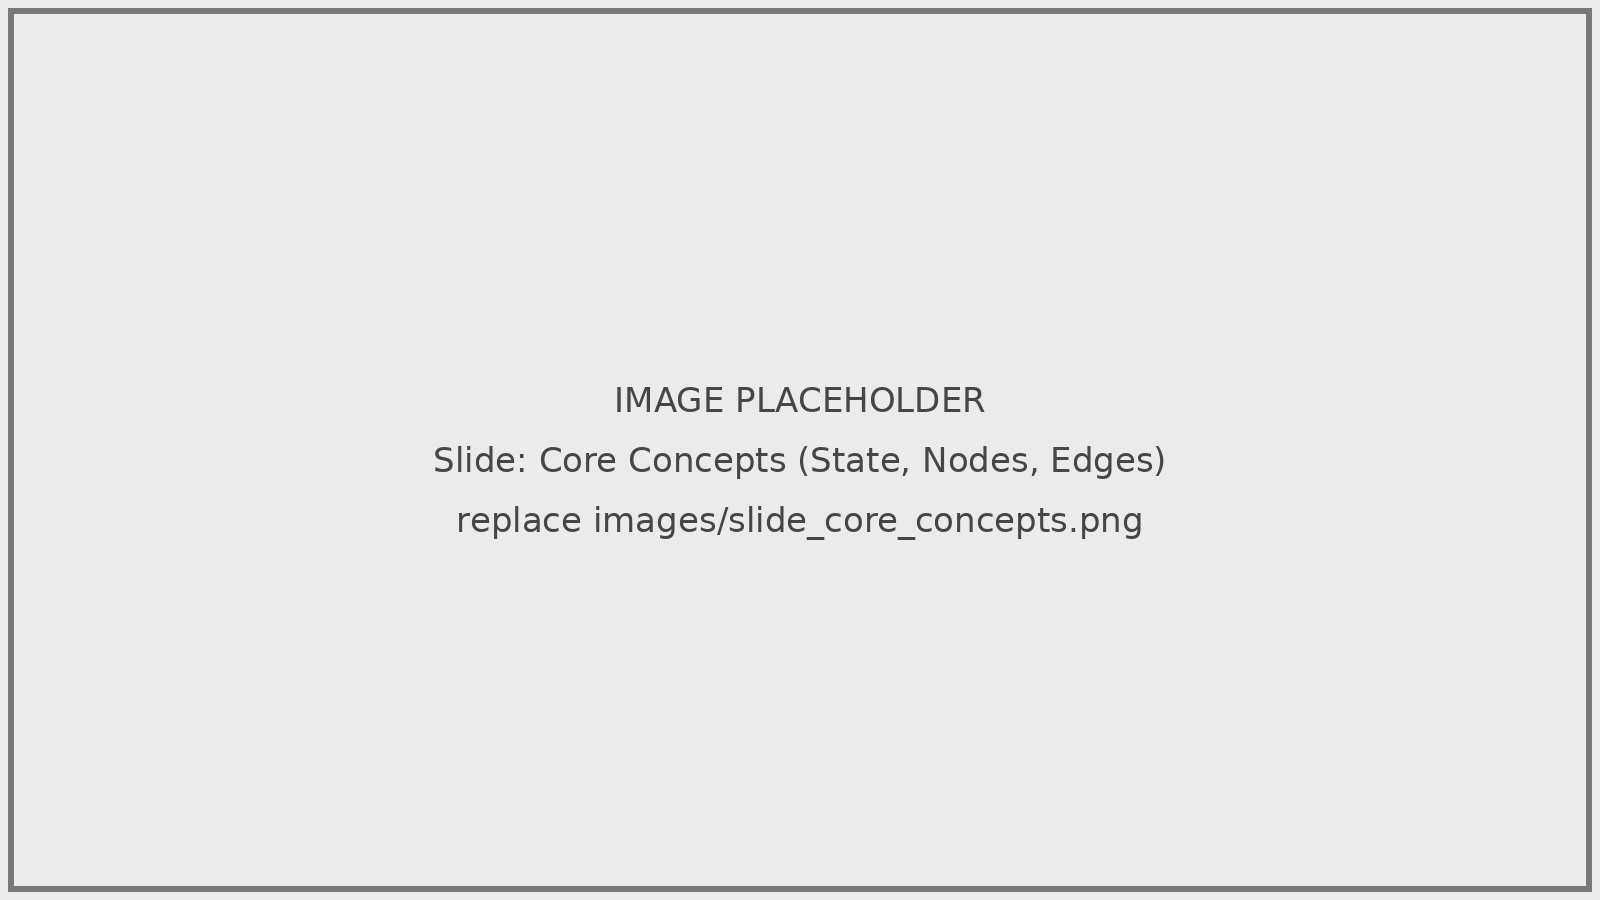
\includegraphics[width=0.85\textwidth]{slide_core_concepts.png}
\caption{Seminar slide: core concepts of LangGraph}
\label{fig:s1}
\end{figure}

\begin{figure}[H]
\centering
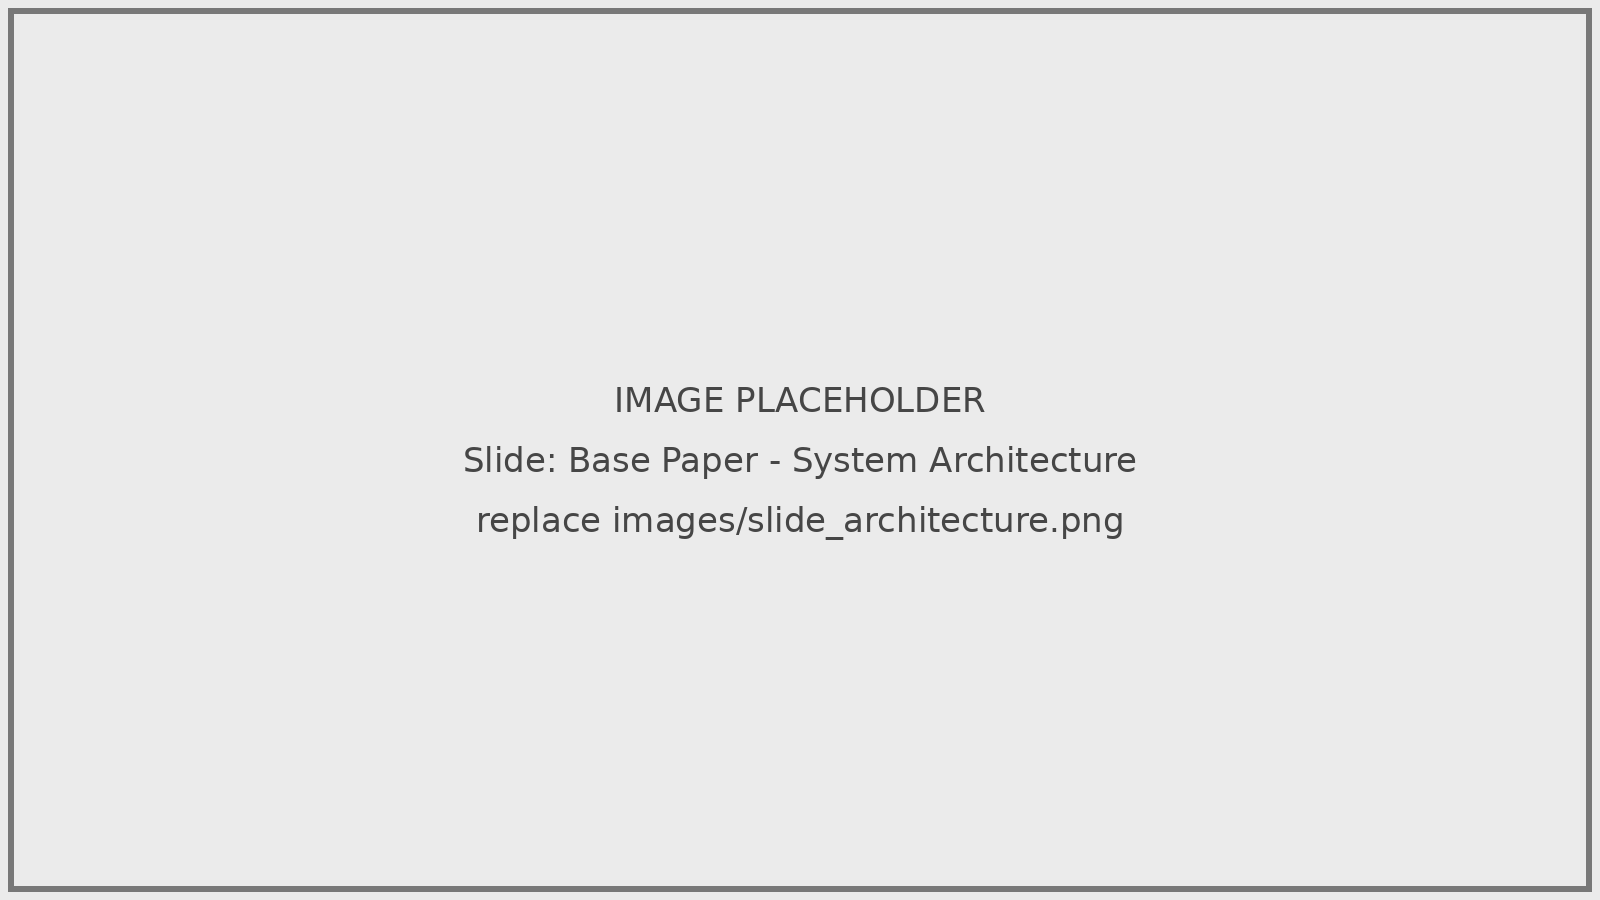
\includegraphics[width=0.85\textwidth]{slide_architecture.png}
\caption{Seminar slide: system architecture of the base paper}
\label{fig:s2}
\end{figure}

\begin{figure}[H]
\centering
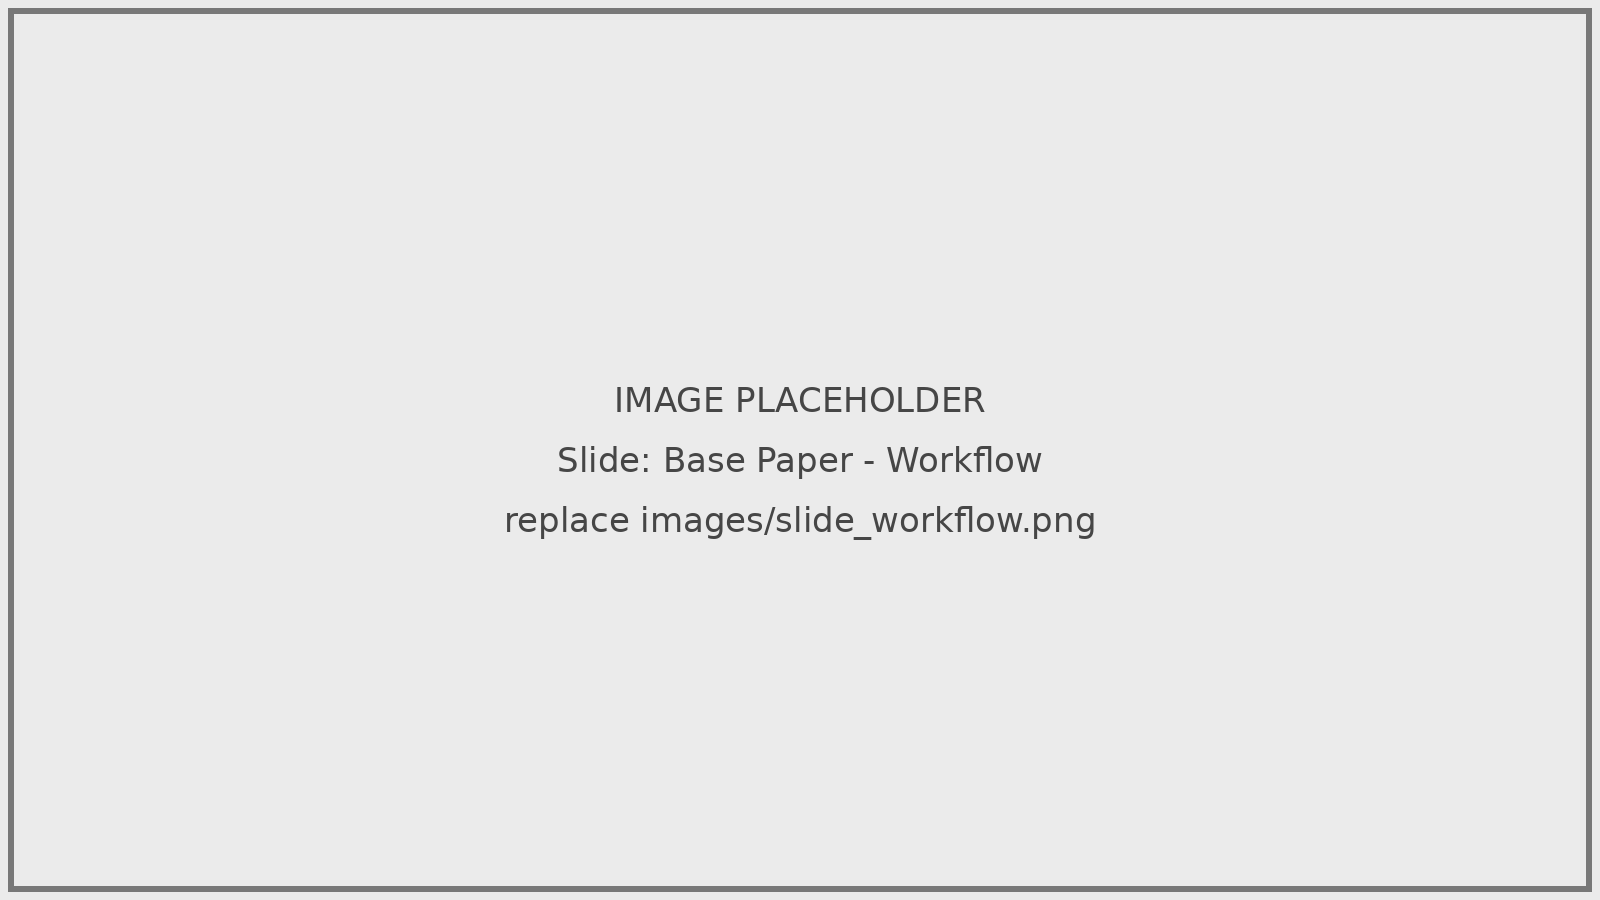
\includegraphics[width=0.85\textwidth]{slide_workflow.png}
\caption{Seminar slide: workflow of the base paper}
\label{fig:s3}
\end{figure}

\begin{figure}[H]
\centering
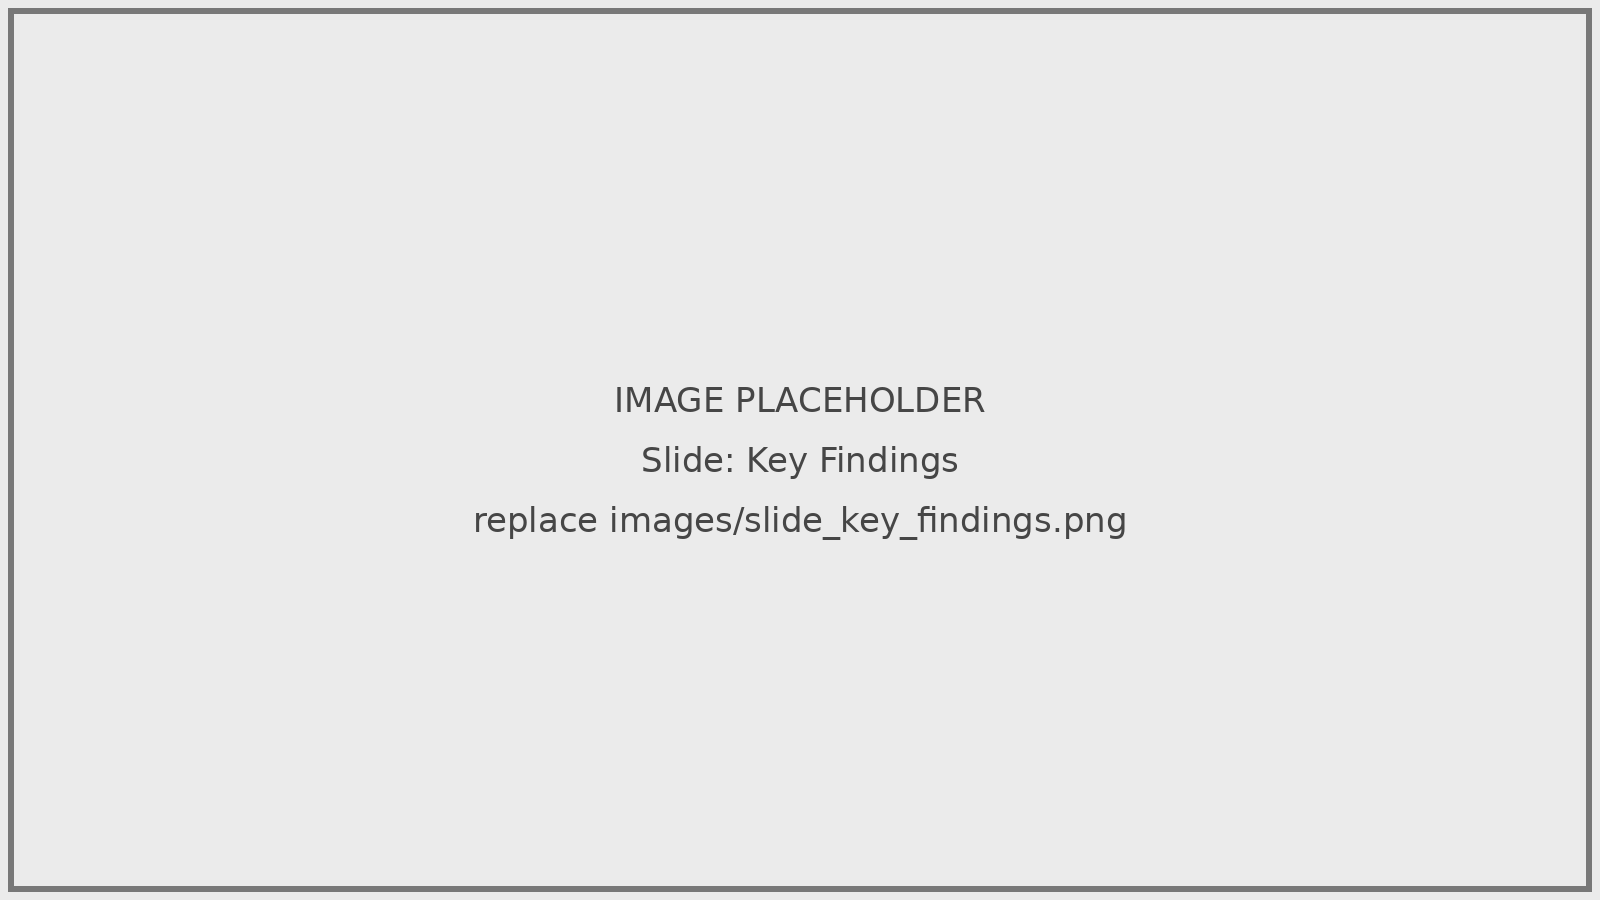
\includegraphics[width=0.85\textwidth]{slide_key_findings.png}
\caption{Seminar slide: key findings}
\label{fig:s4}
\end{figure}

\chapter{Sample Reference Papers}

\begin{figure}[H]
\centering
\fbox{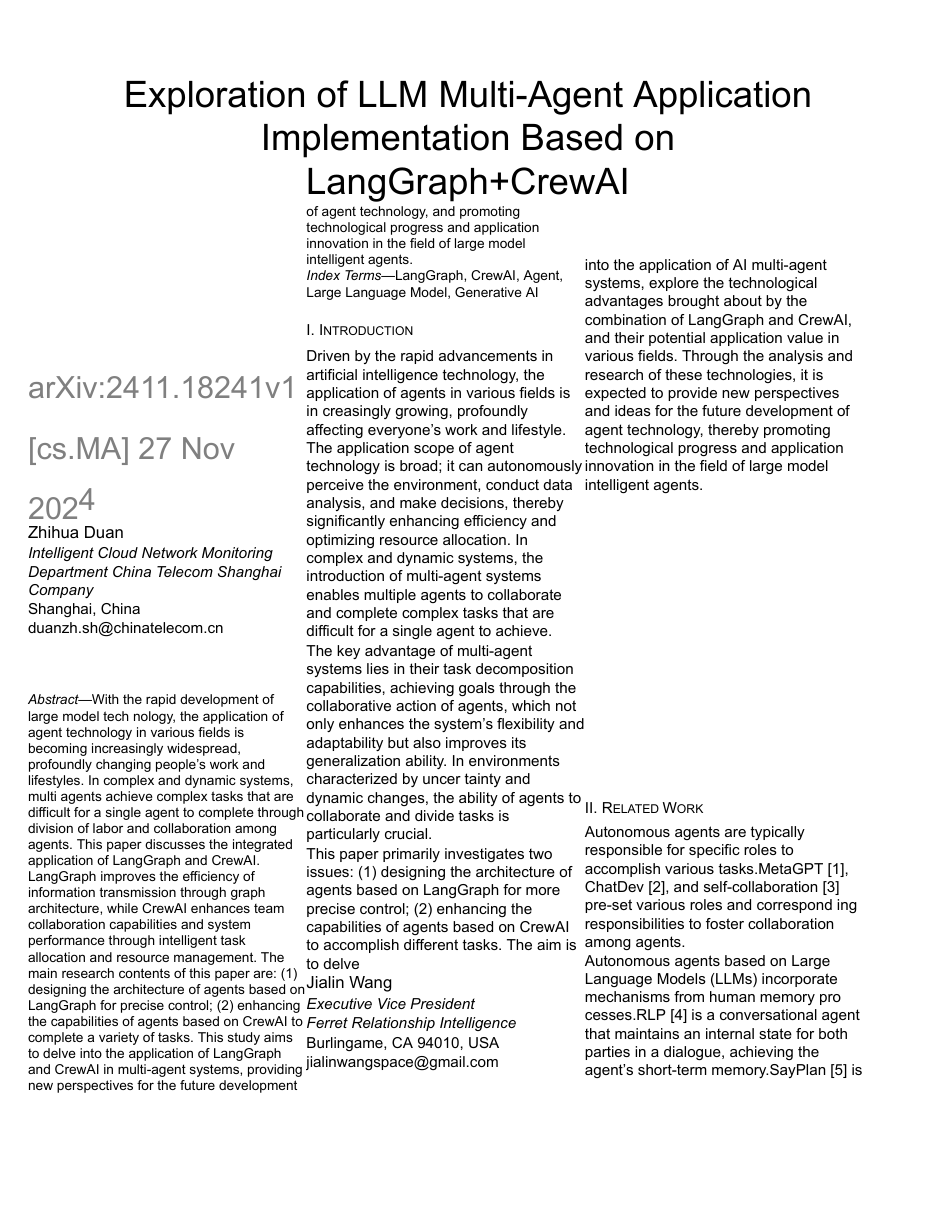
\includegraphics[height=0.62\textheight]{basepaper_p1.png}}
\caption{Base paper: ``Exploration of LLM Multi-Agent Application Implementation Based on LangGraph+CrewAI'' (first page)}
\label{fig:bp}
\end{figure}

\chapter{Viva Questions and Answers}

\subsection*{Common Viva Questions}
\begin{enumerate}[leftmargin=*, itemsep=6pt]
    \item \textbf{What is LangGraph?}\\
    \textit{Answer:} LangGraph is an open-source library from LangChain Inc.\ for building stateful, multi-step LLM applications as a graph of nodes (steps) and edges (transitions) that share one state object.

    \item \textbf{How is LangGraph different from a LangChain chain?}\\
    \textit{Answer:} A chain runs a fixed, one-way sequence of steps. A LangGraph graph can branch with conditional edges, loop back to earlier steps, keep shared state and save checkpoints, so it can retry, pause and resume.

    \item \textbf{What are state, nodes and edges?}\\
    \textit{Answer:} The state is shared data, usually a typed dictionary, that every node reads and updates. A node is a function that performs one step. An edge is a transition between nodes, and a conditional edge uses a router function to choose the next node from the current state.

    \item \textbf{What is a checkpointer and why is it useful?}\\
    \textit{Answer:} A checkpointer saves the graph state after every step. This allows a run to resume after a crash, to be inspected for debugging, and to pause for human approval before continuing.

    \item \textbf{What does CrewAI add to LangGraph in the base paper?}\\
    \textit{Answer:} CrewAI provides role-based teamwork. Agents are defined with roles, goals and tools, and tasks are allocated among them. LangGraph controls the order of steps and the state, while a CrewAI crew performs the work inside a node.

    \item \textbf{Explain the email example from the base paper.}\\
    \textit{Answer:} The graph starts at \texttt{check\_new\_emails}. If there are new emails, it continues to \texttt{draft\_responses}, which runs a CrewAI crew; otherwise it goes to \texttt{wait\_next\_run}. After waiting, it loops back to check again.

    \item \textbf{What tools did the authors use besides LangGraph and CrewAI?}\\
    \textit{Answer:} LangSmith for tracking and auditing workflows, an Ollama embedding model to turn work-order text into vectors, and FAISS as the vector database for fast retrieval.

    \item \textbf{How does LangGraph compare with AutoGen?}\\
    \textit{Answer:} In AutoGen, the flow emerges from the conversation between agents, which is flexible but hard to predict. In LangGraph, the developer defines the allowed paths explicitly, which makes behaviour more controllable and easier to debug.

    \item \textbf{What are the limitations of the base paper?}\\
    \textit{Answer:} The results are qualitative case studies. The paper gives no measurements of accuracy, cost or latency and no comparison with a baseline, so the reported efficiency gains are not yet backed by experiments.

    \item \textbf{Where can LangGraph be applied?}\\
    \textit{Answer:} In customer support routing, RAG question answering, code generation and bug fixing, machine translation, data analysis pipelines, multi-agent research and writing teams, and ticket automation.
\end{enumerate}

\chapter{Similarity Index Report}
[Insert Similarity Index Report Here]

\chapter{Alignment with Sustainable Development Goals (SDG)}

\begin{table}[H]
\centering
\renewcommand{\arraystretch}{1.4}
\caption{Mapping of the seminar topic to relevant UN Sustainable Development Goals (SDGs)}
\label{tab:sdg}
\begin{tabular}{|L{4.5cm}|L{9.5cm}|}
\hline
\textbf{SDG} & \textbf{Rationale for Alignment} \\\hline
SDG 4: Quality Education & Graph-based agents can power tutoring and question-answering assistants, and the clear structure of LangGraph makes agentic AI easier for students to learn. \\\hline
SDG 8: Decent Work and Economic Growth & Automating routine work such as email triage and ticket processing frees people for more meaningful tasks and raises productivity. \\\hline
SDG 9: Industry, Innovation and Infrastructure & Open-source orchestration frameworks lower the barrier to building reliable AI systems, supporting innovation in industry and research. \\\hline
SDG 17: Partnerships for the Goals & Open-source, model-agnostic tools encourage collaboration among researchers, developers and organisations. \\\hline
\end{tabular}
\end{table}

\end{document}
